\documentclass[11pt, letter]{article}

% Load packages
\usepackage[style = authoryear, autocite=inline, doi=false,isbn=false,url=false]{biblatex}
\usepackage[margin = 1 in]{geometry}
\usepackage[colorlinks, citecolor = red]{hyperref}
\usepackage{amsmath, amssymb} %essential
\usepackage[long, nodayofweek]{datetime}
\usepackage[]{booktabs}
\usepackage{graphicx}
\usepackage{setspace}
\usepackage{todonotes}

% Define symbols
\DeclareRobustCommand{\bbone}{\text{\usefont{U}{bbold}{m}{n}1}}
\DeclareMathOperator{\EX}{\mathbb{E}} % expected value
\DeclareMathOperator{\V}{\mathbb{V}}
\DeclareMathOperator{\Prob}{\mathbb{P}}

\begin{document}
\author{Andrew C. Eggers\thanks{Nuffield College and Department of Politics and International Relations, University of Oxford, United Kingdom. \texttt{aeggers@nuffield.ox.ac.uk}}
\and
Tobias Nowacki\thanks{Department of Political Science, Stanford University, CA, United States. \texttt{tnowacki@stanford.edu}}}
\date{\today}
\title{Comparing strategic voting incentives in plurality and instant-runoff elections}

\maketitle

\onehalfspacing % set line space

\section{Data}

To assess the prevalence and distribution of strategic incentives under plurality and IRV empirically, we rely on the Comparative Study of Electoral Systems (CSES) data for a realistic set of preferences and beliefs. The dataset covers 160 surveys from xx different countries, administered shortly before or after an election.\footnote{Two additional cases in the survey, Belarus (20xx) and Lithuania (20xx), are dropped because no respondent specified full preferences over more than two parties.} We focus on the three largest parties (evaluated how?) and label them $A, B, C$ in descending size, respectively. From each survey, we take the party like/dislike scores to approximate voters' ordinal utilities and construct their preference ranking. Let $\bf \tilde{v}$ be the vector of ballot proportions if everyone in the survey voted sincerely. Then, we assume that respondents' beliefs about the next election can be captured with a $\text{Dir}(s \times \bf \tilde{v})$ distribution. Using this set up, we can calculate the strategic incentives under either electoral system as laid out in Section 2.

We should begin with the caveat that a theory that incorporates all relevant parameters (utilities, beliefs, information, etc.) and their respective interactions would be too demanding. Instead, we intend to give our readers a broad sketch of the main theoretical implications; the subsequent presentation of results will address these and explain additional patterns in the data.

\subsection{Summary statistics}

\begin{figure}[!htb]
	\centering
	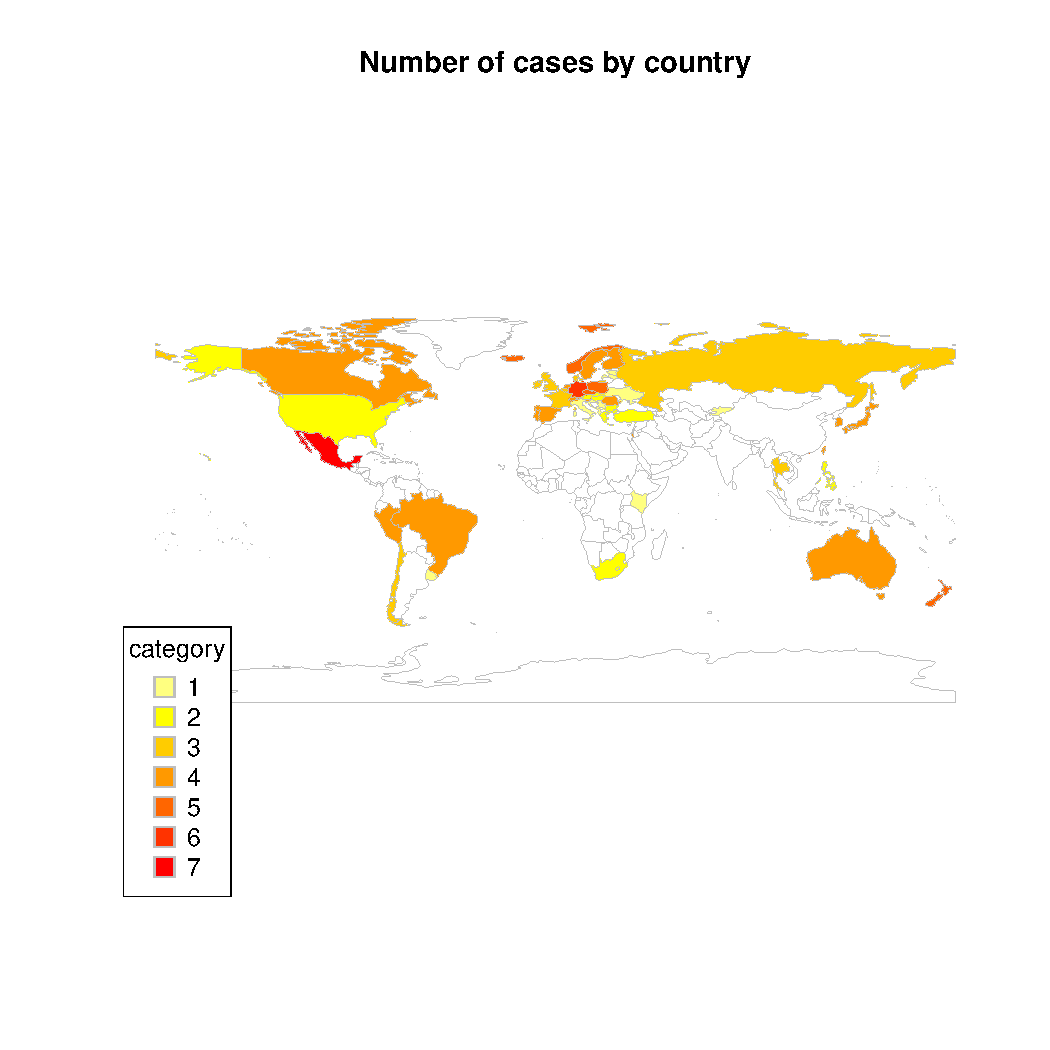
\includegraphics[width = .5 \textwidth]{../output/figures/case_map.pdf}
	\caption{Cases in CSES data, by country}
	\label{fig:case_map}
\end{figure}

The mean number of respondents in each case is 1384 (with a standard deviation of 539). The 160 different surveys come from xx different countries from the time between 1996 and 2016. Figure~\ref{fig:map} maps the number of surveys in each country. (Do we need to say any more? Perhaps something about mean / sd of preference intensity and $\tau$?)

\subsection{Distribution of preferences} 

How different are the CSES cases from one another? Aside from the intensity of preferences, we can describe each case with the vector $\bf \tilde{v}$, where the three-item vector $(v_1 + v_2, v_3 + v_4, v_5 + v_6)$ describes the distribution of first preferences, and the three-item vector $(m_{AB} = \frac{v_1}{v_1 + v_2}, m_{BA} = \frac{v_3}{v_3 + v_4}, m_{CB} = \frac{v_6}{v_5 + v_6})$ describes the distribution of second preferences. 

To link these two distributions together and classify cases more completely, we offer the following approach. Without loss of generality, let the candidate (party) $X$ whose first-preference voters have the most equally split second preferences, and the other two parties $Y$ and $Z$. If both $m_{YZ}$, $m_{ZY} > 0.6$, then classify this case as \emph{single-peaked} and denote it $X+$.\footnote{$X$ is the attractor: both remaining parties have a majority of their second preferences tilted towards $X$.} Conversely, if both $m_{YZ}, m{ZY} < 0.4$, then classify this case as \emph{divided majority} and denote it $X-$.\footnote{Here, $X$ is the repeller: both remaining parties have a majority of their second preferences tilted towards each other and away from $X$.} If $m_{YZ}, m_{ZY} \in [0.4, 0.6]$, then classify this case as \emph{neutral} and denote it $N(X)$. If neither of these conditions hold (because of unusual second preferences), classify it as \emph{other} and denote it $O$. This completes a mutually exclusive and exhaustive set of classes determined by $\bf \tilde{v}$.

\begin{table}[tb]
	\caption{Distribution of preference profiles in CSES data}
	\label{tab:csesprefs}
	\centering

	\begin{tabular}{lccc}
	\hline

	\toprule
	\textbf{} & \textbf{A} & \textbf{B} & \textbf{C} \\
	\cmidrule{2-4}
	Single-peaked (+) & 18 & 23 & 9  \\
	Divided majority (-) & 28 & 20 & 20  \\
	Neutral () & 5 & 7 & 3  \\
	Other () & & 27 &  \\
	\bottomrule
	\end{tabular}
\end{table}

Table~\ref{tab:csesprefs} summarises the distribution of preference classes across the CSES cases. A plurality of cases belong to the divided majority classes; however, there is also a large number of single-peaked cases, whereas neutral and others tend to be rarer. (Figure~\ref{fig:cses_fp} plots the distribution of first preferences conditional on the classes.)

\begin{figure}[!htb]
	\centering
	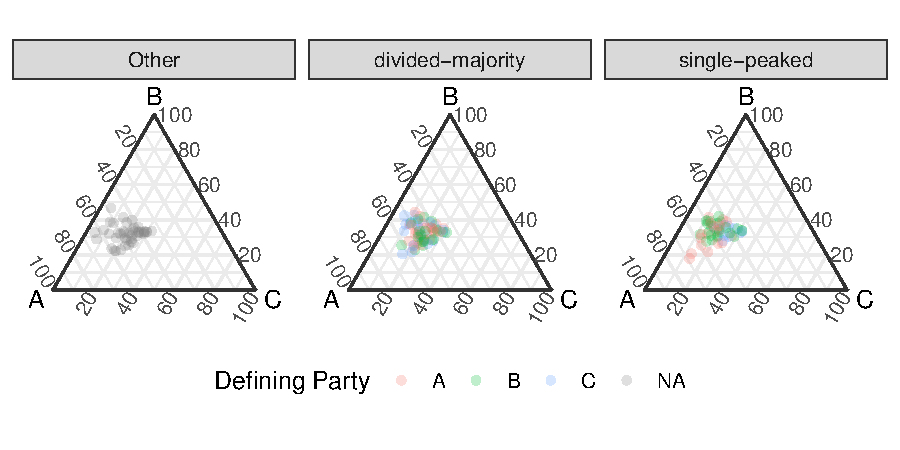
\includegraphics[width = 0.6 \textwidth]{../output/figures/cses_fp.pdf}
	\caption{Distribution of first preferences in CSES cases, by class}
	\label{fig:cses_fp}
\end{figure}

\section{Results: Baseline Case}

\subsection{Theoretical intuition}

\emph{The current draft does not introduce the reader to IRV mechanisms or types of votes at all. Should it? Or perhaps this is a better place for it.}

Our main objective in this section is to evaluate and compare IRV and Plurality, given the set of preferences and beliefs from the CSES, along two criteria: the prevalence of strategic incentives (the proportion of respondents with $\tau > 0$) and the magnitude of such incentives (the distribution and range of $\tau$). 

We expect strategic incentives to be more prevalent under IRV than under Plurality. Under the latter, the only strategic incentive that can exist is if you believe that your first preference comes third; you will want to vote for one of the two front-runners instead. Under IRV, this is different -- there are many more pivotal events (both first-round and second-round) happening. (For example, even if my first preference is leading in the expected result, I may still want to vote strategically to prevent them from being beaten in the second round). It is, of course, possible to come up with existence proofs of $
\bf U$ such that the prevalence of strategic incentives is bigger under plurality than under IRV, but we expect those cases to be much rarer (why?).

(\emph{What about $s$?}) Furthermore, we expect strategic incentives to be much more sensitive to the precision of beliefs, defined by the parameter $s$, under IRV. Under Plurality, there is only one out of three pivotal events that would justify strategic voting; intutively, I merely need to know about the expected order of finish and how likely it is that my first preference ends up in the top two. (Can we re-write $\tau_{plur}$ as a function of the probability of coming within the top two?) This is much more complex under IRV: not only are there more pivotal events, but they also point towards different strategic votes (an $ABC$ voter could vote $BAC$ or $CAB$ instead).\footnote{Note that although possible, it \emph{never} makes sense for a voter to rank their first preference last. This is because doing so would mean helping a less-prefered candidate in any pivotal event that includes the first preference.}

\subsection{Prevalence of Strategic Incentives}

Figure~\ref{fig:sv_dist} plots all CSES cases according to their proportion of voters with strategic incentives under both IRV ($\Prob(\tau_{IRV} > 0)$) and Plurality ($\Prob(\tau_{plur} > 0)$), at various levels of information precision. Data points below the 45 degree line have a greater proportion of voters with positive strategic incentives under plurality than under IRV; the reverse is true for cases above the 45 degree line.

\begin{figure}[!h]
	\centering
	\includegraphics[width = .8 \textwidth]{"../output/figures/cses_prop"}
	\caption{Proportion of voters with positive strategic incentive under Plurality and IRV}
	\label{fig:sv_dist}
\end{figure}

What is immediately striking in Figure~\ref{fig:sv_dist} is that the proportion under plurality seems capped at about 0.2, independent of belief precision. These cases may constitute a `worst-case' scenario for voters who have the third-placed party as their first preference: they are numerous enough to make up a fifth of the population, but are still few enough that, acting optimally, they should abandon their first preference and flock to one of the two main parties instead.\footnote{Of course, this also depends on the distribution of preference intensity. A voter with the utility vector $(10, 2, 1)$ will need a much more 'hopeless' scenario than one who is almost indifferent between first and second preference (e.g., $(10, 9, 1)$).} (At expected vote shares $> 0.2$, the three parties would be reasonably close to each other and it would be better for party supporters to stick to their first preference.)

The other notable trend in Figure~\ref{fig:sv_dist} is that as $s$ increases, the proportion of voters with positive strategic incentives under IRV rises in some, but not all cases. With reasonably precise beliefs ($s > 75$), there is a subgroup of cases that exhibits very high prevalence of strategic incentives under IRV with around (and sometimes even more than) half of the voters. Equally, there is a cluster of cases where the overall incentives under IRV do not change much, these cases remain distributed tightly along the 45-degree line. (For a summary, see Table~\ref{tab:strat_inc})

\begin{table}[!htb]
	\caption{Number of cases where IRV incentive is greater}
	\label{tab:strat_inc}
	\centering

	\begin{tabular}{lccc}
	\toprule
	s & \textbf{IRV $>$ Plur} & \textbf{IRV $<$ Plur} & \textbf{Proportion IRV $>$ Plur} \\
	\cmidrule{2-4}
	15 & 41 & 119 & 0.256 \\
	30 & 58 & 102 & 0.362 \\
	45 & 66 & 94 & 0.412 \\
	60 & 73 & 87 & 0.456 \\
	75 & 83 & 77 & 0.519 \\
	85 & 88 & 72 & 0.550 \\
	90 & 90 & 70 & 0.563 \\
	\bottomrule
	\end{tabular}
\end{table}

This result emphasises the importance of modelling realistic preferences and beliefs to check for meaningful results on strategic incentives. While we cannot conclude that the prevalence of strategic incentives under IRV will \emph{always} be higher (such a claim would be theoretically impossible), this result supports the claim that the \emph{expected} prevalence of strategic incentives will be higher under IRV (given our assumptions about likely preference profiles.)

\subsection{Magnitude of Strategic Incentives}

The next question is how strong these incentives are: the magnitude of $\tau$ indicates the magnitude of the expected benefit when compared to a sincere ballot. Theoretically, we expect incentives to be greater under Plurality because of the lower complexity of strategic situations; under IRV, in contrast, there are multiple pivotal events where the same submitted ballot can have opposite effects; thus, the benefit of some strategic actions may be attenuated by the probability of them backfiring.

(Example here?)

\begin{figure}[!h]
	\centering
	\includegraphics[width = .8 \textwidth]{"../output/figures/epsilon_true_scale"}
	\caption{Difference in proportion of voters with strategic incentive $\tau \geq \varepsilon$}
	\label{fig:sv_epsilon}
\end{figure}

Figure~\ref{fig:sv_epsilon} plots the mean difference, along with standard errors, in the proportion of voters with a strategic incentive that is greater than some threshold value $\epsilon$.\footnote{Explain how we aggregated different cases, weighted by electoral population and sample size.} Positive differences indicate that there are more voters under IRV than under Plurality who have a $\tau \geq \varepsilon$). This is only true for very small values of $\epsilon$, but the difference decreases rapidly and then turns negative. This supports our theoretical claim that, although the total prevalence of strategic incentives is higher under IRV, much of it is due to very small incentives.

One way to think about the importance of this result is to interpret $\varepsilon$ as a constant cost of strategic voting; this may be due to the need for more complex calculations, or simply the opportunity cost of not casting an expressive vote for one's first preference. This implies that there is a bigger group of voters who have a lot to gain from voting strategically under Plurality, whereas the benefits of doing so under IRV are possibly consumed by the need for strategic calculations in the first place.\footnote{A voter who considers a `strong pushover' vote, for example, will have to carefully form a prior about the likelihood of such a ballot accidentally electing their third preference. This kind of trade-off is much easier under Plurality due to the restricted number of pivotal events.} Extending further, this may be a possible reason for why we observe strategic voting in Plurality, but rarely and non-systematically under IRV (and hence giving rise to statements such as that by Nick Clegg that strategic voting under IRV is `impossible'). Investigating such a hypothesis, however, is a task for future research.

\subsection{Condorcet Winner}

A simple way to evaluate the aggregate performance of the two electoral systems is to check how often, given the distribution of true preferences, the Condorcet Winner is elected if a proportion $\lambda$ of the population votes strategically. 

To that end, we compute...

Figure~\ref{fig:sv_condor} summarises the result.

\begin{figure}[!h]
	\centering
	\includegraphics[width = .8 \textwidth]{"../output/figures/condorcet_probs"}
	\caption{Probability of the Condorcet Winner being elected under either Plurality or IRV}
	\label{fig:sv_condor}
\end{figure}




\section{Results: Interdependence of Strategic Behaviour}

\end{document}